\documentclass[a4paper,11pt]{article}
\usepackage{amsmath,amsthm,amssymb}
\usepackage{mathtools}
\usepackage{mathrsfs}
\usepackage{setspace}
\usepackage{enumerate}
\usepackage{caption}
\DeclarePairedDelimiter\abs{\lvert}{\rvert}
\PassOptionsToPackage{usenames,dvipsnames,svgnames}{xcolor}  
\usepackage{tikz}
\usetikzlibrary{arrows,positioning,automata,fit,shapes,backgrounds}
\usepackage{framed}
\begin{document}
\newtheorem*{theorem1}{Theorem}
\newtheorem*{theorem2}{Theorem}
\newtheorem*{theorem3}{Theorem}
\newtheorem*{theorem4}{Theorem}
\newtheorem*{theorem5}{Theorem}
\newtheorem*{theorem6}{Theorem}
\newtheorem*{theorem7}{Theorem}
\newtheorem*{theorem8}{Theorem}
\newtheorem*{theorem9}{True/False?}
\title{MATH 393 Week 8 Assignment 2\textsuperscript{nd} Draft}
\author{Brett Bonner}
\date{March 8, 2014}
\maketitle
\doublespacing
\newcounter{ProblemCounter}
\newcounter{SubsectionCounter}[ProblemCounter]
\addtocounter{ProblemCounter}{6} % set them to some other numbers than 0
\addtocounter{SubsectionCounter}{3} % same
%

\setcounter{ProblemCounter}{6}
\section*{\S 2.5 Exercise \arabic{ProblemCounter}: Use the PCI to prove the following properties of Fibonacci numbers:}
\setcounter{SubsectionCounter}{4}
\textbf{\arabic{ProblemCounter}.\alph{SubsectionCounter}}
(Binet's formula) Let \(\alpha\) be the positive solution and \(\beta\) the negative
solution to the equation \(x^2 = x + 1\). (The values are \(\alpha = \frac{1 + \sqrt{5}}{2}\) 
and\\
\(\beta = \frac{1-\sqrt{5}}{2}\).)
Show for all natural numbers \(n\) that
 \(f_n=\frac{\alpha^n-\beta^n}{\alpha - \beta}\)
\begin{theorem1}
\(f_n=\frac{\alpha^n-\beta^n}{\alpha - \beta}\) for all natural numbers \(n\).
 \begin{proof}
Let S = \(\{n : f_n= \frac{\alpha^2-\beta^2}{\alpha - \beta}\}\)
As \(\alpha\) and \(\beta\) are the positive and negative roots, respectively, for 
the equation \(x^2-x-1=0\). Therefore:\\
\(\alpha^2-\alpha-1=0 \therefore \alpha^2=\alpha+1\)\\
\(\beta^2-\beta-1=0 \therefore \beta^2=\beta+1\)
\begin{enumerate}[(i)]   
 \item To show the base case \(n=1 \in S\), we must show \(f_1=1\) and \(f_2=1\).\\
 \(f_1 = \frac{\alpha^1-\beta^1}{\alpha-\beta} = 1\)\\
 \(f_2 = \frac{\alpha^2 - \beta^2}{\alpha-\beta} = \frac{{(\alpha+1)} - {(\beta+1)}}{\alpha-\beta} = \frac{\alpha - \beta}{\alpha-\beta} = 1\)
 \newpage
 \item To show \(n \in S\), assume \(1, 2 \ldots n-1 \in S\)\\
 Show that \(f_{n} = \frac{\alpha^n-\beta^n}{\alpha - \beta}\)
 \begin{alignat*}{3}
   f_n &= f_{n-1}+f_{n-2}\\
   \cdots &= \frac{\alpha^{n-1}-\beta^{n-1}}{\alpha - \beta} + \frac{\alpha^{n-2}-\beta^{n-2}}{\alpha - 
   \beta}\\
   \cdots &= \frac{\alpha^{n-1}-\beta^{n-1} + \alpha^{n-2}-\beta^{n-2}}{\alpha - 
   \beta}\text{ factoring }\alpha \text{ and }\beta \text{ from the numerator}\ldots\\
   \cdots &= \frac{{(\alpha + 1){(\alpha^{n-2})}}-{(\beta + 1)}{(\beta^{n-2})}}{\alpha - 
   \beta}\\
   &\text{As }\alpha+1 = \alpha^2 \text{ and }\beta+1 = \beta^2 \text{ we 
   substitute}\ldots\\
   \cdots &= \frac{{(\alpha^2){(\alpha^{n-2})}}-{(\beta^2)}{(\beta^{n-2})}}{\alpha - 
   \beta}\\
   f_n &= \frac{\alpha^n-\beta^n}{\alpha - \beta}\\
   \text{Thus } n \in S
 \end{alignat*}
 \item As \(n \in S\) we conclude that for all natural numbers \(n\) that \(f_n=\frac{\alpha^n-\beta^n}{\alpha - 
 \beta}\) by the PCI.
\end{enumerate}
\end{proof}  
\end{theorem1}
\newpage

\setcounter{ProblemCounter}{11}
\section*{\S 2.5 Exercise \arabic{ProblemCounter}: Let the ``Fibonacci-2'' numbers \(g_n\) be defined as follows:}
\(g_1=2, g_2=2, g_{n+2}=g_{n+1}g_n\) for all \(n \geq 1\)\\\\
\setcounter{SubsectionCounter}{1}
\textbf{\arabic{ProblemCounter}.\alph{SubsectionCounter}}
Calculate the first five ``Fibonacci-2'' numbers.\\
\begin{alignat*}{3}
  g_1 &= 2\\
  g_2 &= 2\\
  g_3 &= {(g_2)}{(g_1)} &= 4\\
  g_4 &= {(g_3)}{(g_2)} &= 8\\
  g_5 &= {(g_4)}{(g_3)} &= 32
\end{alignat*}
\newpage
\section*{\S 2.5 Exercise \arabic{ProblemCounter}: Let the ``Fibonacci-2'' numbers \(g_n\) be defined as follows:}
\(g_1=2, g_2=2, g_{n+2}=g_{n+1}g_n\) for all \(n \geq 1\)\\
\setcounter{SubsectionCounter}{2}
\noindent\textbf{\arabic{ProblemCounter}.\alph{SubsectionCounter}}
Show that \(g_n=2^{f_{n}}\).
\begin{theorem1}
  \(g_n=2^{f_{n}}\) where \(f_n = f_{n-1} + f_{n-2}\)
  \begin{proof}
    Let \(S = \{n \in \mathbb{N}: g_n = 2^{f_n}\}\)
    \begin{enumerate}[(i)]
      \item Let \(n=1\), then \(g_1 = 2^{f_1} = 2\).\\
      Let \(n =2 \), then \(g_2 = 2^{f_2} = 2\).\\
      Thus \(1 \in S\) and \(2 \in S\).
      \item Now show that \(\{1, 2, 3\ldots n-1\} \subseteq S \Rightarrow n \in 
      S\) where \(n > 2\).\\
      Assume \(\{1,2,3\ldots n-1 \subseteq S\}\), \(n-1 \in S\) and \(n-2 \in 
      S\).\\
      As \(n-1 \in S\), then \(g_{n-1}=2^{f_{n-1}}\).\\
      As \(n-2 \in S\), then \(g_{n-2}=2^{f_{n-2}}\)\\
      To show \(g_n = 2^{f_{n}}\):
      \begin{alignat*}{3}
        g_n &= g_{n-1}g_{n-2}\\
        \cdots &= {(2^{f_{n-1}})}{(2^{f_{n-2}})}\\
        \cdots &= 2^{f_{n-1}+f_{n-2}} \text{ and since } f_n = f_{n-1} + f_{n-2}\ldots\\
        g_n &= 2^{f_{n}}
      \end{alignat*}
      Therefore \(n \in S\) and therefore we have shown by PCI \(g_n = 2^{f_{n}}\).
    \end{enumerate}
  \end{proof}
\end{theorem1}
\newpage

\setcounter{ProblemCounter}{1}
\section*{\S 2.5 Exercise \arabic{ProblemCounter}: Let \(T\) be the relation\\ \{{(3,1)},{(2,3)},{(3,5)},{(2,2)},{(1,6)},{(2,6)},{(1,2)}\}. Find}
\setcounter{SubsectionCounter}{1}
\textbf{\arabic{ProblemCounter}.\alph{SubsectionCounter}}
Dom {(\(T\))}.\\
Dom {(\(T\))} = \{1,2,3\}\\
\addtocounter{SubsectionCounter}{1}
\textbf{\arabic{ProblemCounter}.\alph{SubsectionCounter}}
Rng {(\(T\))}.\\
Rng {(\(T\))} = \{1,2,3,5,6\}.\\
\addtocounter{SubsectionCounter}{1}
\textbf{\arabic{ProblemCounter}.\alph{SubsectionCounter}}
\(T^{-1}\).\\
\(T^{-1}\) = \{{(1,3)},{(3,2)},{(5,3)},{(2,2)},{(6,1)},{(6,2)},{(2,1)}\}.\\
\addtocounter{SubsectionCounter}{1}
\textbf{\arabic{ProblemCounter}.\alph{SubsectionCounter}}
\({(T^{-1})}^{-1}\).\\
\({(T^{-1})}^{-1}\) = \(T\) = \{{(3,1)},{(2,3)},{(3,5)},{(2,2)},{(1,6)},{(2,6)},{(1,2)}\}.\\
\newpage

\setcounter{ProblemCounter}{7}
\section*{\S 3.1 Exercise \arabic{ProblemCounter}: Give the digraphs for these relations on the set \(\{1,2,3\}\)}
\setcounter{SubsectionCounter}{2}
\textbf{\arabic{ProblemCounter}.\alph{SubsectionCounter}}
\(S=\{{(1,3)},{(2,1)}\}\)\\
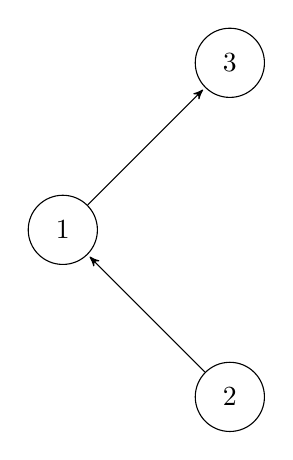
\begin{tikzpicture}[>=stealth',shorten >=1pt,node distance=3cm,on grid,initial/.style ={}]
  \node[state]          (1)                        {$1$};
  \node[state]          (3) [above right =of 1]    {$3$};
  \node[state]          (2) [below right =of 1]    {$2$};
\tikzset{mystyle/.style={->}} 
\tikzset{every node/.style={fill=none}} 
\path (1)     edge [mystyle]    node   {} (3)
      (2)     edge [mystyle]    node   {} (1);
\end{tikzpicture}\\
\setcounter{SubsectionCounter}{4}
\textbf{\arabic{ProblemCounter}.\alph{SubsectionCounter}}
\(S^{-1}\) where \(S=\{{(1,3),{(2,1)}\}\)\\
\(S^{-1} = \{{(3,1),{(1,2)}}\}\)\\
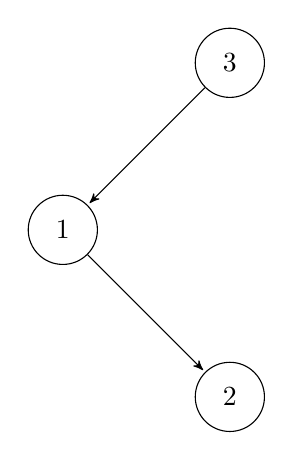
\begin{tikzpicture}[>=stealth',shorten >=1pt,node distance=3cm,on grid,initial/.style ={}]
  \node[state]          (1)                        {$1$};
  \node[state]          (3) [above right =of 1]    {$3$};
  \node[state]          (2) [below right =of 1]    {$2$};
\tikzset{mystyle/.style={->}} 
\tikzset{every node/.style={fill=none}} 
\path (3)     edge [mystyle]    node   {} (1)
      (1)     edge [mystyle]    node   {} (2);
\end{tikzpicture}\\
\setcounter{SubsectionCounter}{6}
\newpage
\section*{\S 3.1 Exercise \arabic{ProblemCounter}: Give the digraphs for these relations on the set \(\{1,2,3\}\)}

\textbf{\arabic{ProblemCounter}.\alph{SubsectionCounter}}
\(S \circ S \) where \(S=\{{(1,3),{(2,1)}\}\)\\
\begin{figure}[h!]
\begin{framed}
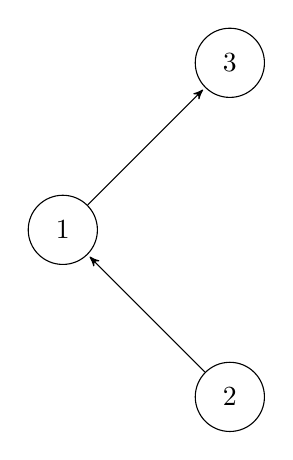
\begin{tikzpicture}[>=stealth',shorten >=1pt,node distance=3cm,on grid,initial/.style ={}]
  \node[state]          (1)                        {$1$};
  \node[state]          (3) [above right =of 1]    {$3$};
  \node[state]          (2) [below right =of 1]    {$2$};
\tikzset{mystyle/.style={->}} 
\tikzset{every node/.style={fill=none}} 
\path (1)     edge [mystyle]    node   {} (3)
      (2)     edge [mystyle]    node   {} (1);
\end{tikzpicture}
\captionsetup{justification=raggedright,
singlelinecheck=false,margin=3cm}
  \caption*{\(S=\{{(1,3)},{(2,1)}\}\)}
  \end{framed}
\end{figure}
\begin{figure}[htbp!]
\begin{framed}
\begin{tikzpicture}[>=stealth',shorten >=1pt,node distance=3cm,on grid,initial/.style ={}]
  \node[state]          (1)                        {$1$};
  \node[state]          (3) [above right =of 1]    {$3$};
  \node[state]          (2) [below right =of 1]    {$2$};
\tikzset{mystyle/.style={->}} 
\tikzset{every node/.style={fill=none}} 
\path (2)     edge [mystyle]    node   {} (3);
\end{tikzpicture}
\captionsetup{justification=raggedright,
singlelinecheck=false,margin=3cm}
  \caption*{\(S=\{{(1,3)},{(2,1)}\}\), as \({(2,1)}\in S\) and \({(1,3)} \in S\), \(S \circ S = \{(2,3)\}\)}
\end{framed}
\end{figure}
\newpage
\setcounter{ProblemCounter}{9}
\section*{\S 3.1 Exercise \arabic{ProblemCounter}: Let \(R\) be a relation from \(A\) to \(B\) and \(S\) be a relation from \(B\) to \(C\).}
\setcounter{SubsectionCounter}{1}
\textbf{\arabic{ProblemCounter}.\alph{SubsectionCounter}}
Prove that Dom \({(S \circ R)} \subseteq \text{Dom } {(R)}\)
\begin{theorem1} If \(R\) is a relation from \(A\) to \(B\) and \(S\) is a relation from \(B\) to \(C\), Dom \({(S \circ R)} \subseteq \text{Dom } {(R)}\)
  \begin{proof}
    Suppose that \(A , B\) and \(C\) are sets and \(R\) is a relation from \(A\) to \(B\), and \(S\) is a relation from \(B\) to 
    \(C\).\\
    To prove Dom\({(S \circ R)} \subseteq\) Dom \({(R)}\), we must show\\ \(x \in\) 
    Dom\({(S \circ R)} \Rightarrow x \in\) Dom\({(R)}\) for all \(x\).\\
    Let \(x\) be arbitrary and \(x \in {(S \circ R)}\).\\
    Then there exists a \(y \in C\) such that \({(x,y)}\in{(S \circ R)}\).\\
    Then there exists a \(z \in B\) such that \({(x,z)}\in R\) and \({(z,y)}\in 
    S\).\\
    Therefore \(x \in\) Dom\({(R)}\).\\
    Therefore if \(R\) is a relation from \(A\) to \(B\) and \(S\) is a relation from \(B\) to \(C\), Dom\({(S \circ R)}\subseteq\) Dom\({(R)}\).
  \end{proof}
\end{theorem1}
\newpage
\section*{\S 3.1 Exercise \arabic{ProblemCounter}: Let \(R\) be a relation from \(A\) to \(B\) and \(S\) be a relation from \(B\) to \(C\).}
\setcounter{SubsectionCounter}{2}
\noindent\textbf{\arabic{ProblemCounter}.\alph{SubsectionCounter}}
Show by example that Dom \({(S \circ R)} = \text{Dom } {(R)}\) may be false\\
Let \(A=\{\text{What my mom thinks I do},\text{What society thinks I do},\text{What I actually 
do}\}\)..\\
\(B=\{\text{Albert Einstein},\text{Good Will Hunting},\text{Computer Geek}\}\)\\
\(C=\{\text{Physicist},\text{Mathematician},\text{Programmer}\}\)\\
R=\{{(\text{What my mom thinks I do, Albert Einstein})},{(\text{What society thinks I do, Good Will Hunting})},\\{(\text{What I actually do, Computer 
Geek})}\}\\
S=\{{(\text{Albert Einstein, Physicist})},{(\text{Albert Einstein, Mathematician})},\\{(\text{Computer Geek, Programmer})}\}\\
Therefore \ldots:\\
\({(S \circ R)}=\)\{(What my mom thinks I do, Physicist),(What my mom thinks I do, Mathematician), (What I actually do, 
Programmer)\}\\
Dom\({(R)}\)=\{What my mom thinks I do,What society thinks I do,What I actually 
do\}\\
Dom\({(S \circ R)}=\)\{What my mom thinks I do,What I actually 
do\}\\
Therefore by counterexample Dom \({(S \circ R)} \neq \text{Dom } {(R)}\) \(\Box\).
\newpage

\setcounter{ProblemCounter}{10}
\section*{\S 3.1 Exercise \arabic{ProblemCounter}: Complete the proof of Theorem 3.1.3:}
\setcounter{SubsectionCounter}{1}
\textbf{\arabic{ProblemCounter}.\alph{SubsectionCounter}}
\begin{theorem1}
If \(A\) and \(B\) are sets and \(R\) is the relation between \(A\) and \(B\), \({({R^{-1}})}^{-1}=R\)
\begin{proof}
\begin{align*}
{(R^{-1})}^{-1} &= R\\
&\Leftrightarrow {(R^{-1})}^{-1} \subseteq R \text{ and } R \subseteq {(R^{-1})}^{-1}\\
&\Leftrightarrow (x,y) \in {(R^{-1})}^{-1} \Rightarrow {(y,x)}\in {({R^{-1}})}\\
&\Leftrightarrow (x,y) \in R
\end{align*}
\end{proof}  
\end{theorem1}
\newpage
\setcounter{SubsectionCounter}{4}
\section*{\S 3.1 Exercise \arabic{ProblemCounter}: Complete the proof of Theorem 3.1.3:}
\noindent\textbf{\arabic{ProblemCounter}.\alph{SubsectionCounter}}
\({(S \circ R)}^{-1} = R^{-1} \circ S^{-1}\).
\begin{theorem1}
If \(A\), \(B\), and \(C\) are sets and \(R\) is the relation from \(A\) to \(B\) 
and \(S\) is the relation from \(B\) to \(C\), \({(S \circ R)}^{-1} = R^{-1} \circ S^{-1}\)
\begin{proof}
\begin{align*}
{(S \circ R)}^{-1} &= R^{-1} \circ S^{-1}\\
&\Leftrightarrow {(S \circ R)}^{-1} \subseteq R^{-1} \circ S^{-1}
\text{ and } R^{-1} \circ S^{-1} \subseteq {(S \circ R)}^{-1}\\
&\Leftrightarrow {(z,x)} \in {(S \circ R)}^{-1}\\
&\Leftrightarrow {(x,z)} \in S \circ R\\
&\Leftrightarrow {(x,y)} \in R \text{ and } {(y,z)} \in S\\
&\Leftrightarrow {(y,x)} \in R^{-1} \text{ and } {(z,y)} \in S^{-1}\\
&\Leftrightarrow {(z,x)} \in R^{-1} \circ S^{-1}
\end{align*}
\end{proof}  
\end{theorem1}
\end{document}